\documentclass{article}
\usepackage[utf8]{inputenc}

\title{CSE 222A PROJECT - GROUP 6}

\author{Stanislav Mushits, Sreejith Unnikrishnan, Ruby Pai, Amit Borase, Ritvik Jaiswal }
\date{November 24 2015}

\usepackage{natbib}
\usepackage{graphicx}
\usepackage{geometry}
 \geometry{
      a4paper,
           total={170mm,257mm},
            left=20mm,
             top=20mm,
              }

\begin{document}

\maketitle

\begin{center}
\textbf{Coflow scheduler performance verification}
\end{center}

\begin{center}
\textbf{Milestone report 2}
\end{center}

\section{Progress so far}
As part of this milestone, we have completed the following tasks.
\begin{itemize}
	\item Implemented the actor program to create connections between mappers and reducers and start the simulation
	\item Deploying the master and slave programs on individual mininet hosts, and writing a script to automate this task
	\item Running varys simulation on a single Mininet\cite{mininet} host and traditional (without running varys code) simulation on multiple mininet hosts
\end{itemize}
The current state of the project is as follows-
\begin{itemize}
	\item Current simulation involves sending fake data from mapper to reducer.
	\item The Master is the controller which creates connections between mappers and reducers, and starts the simulation.
	\item The Slaves are either mappers or reducers.
	\item The Master reads the simulation file which contains the location of the hosts and task files and a field to specify whether the simulation is a traditional one or a varys simulation, and the task file which contains information about all the mappers and reducers and how much data each mapper sends to a reducer.
	\item Based on this, the connections between mappers and reducers is established, and the simulation is started.
\end{itemize}
\subsection{Varys simulation}
\begin{itemize}
	\item A single mininet host runs the Master and Slaves along with the varys\cite{varys} scheduler running on the controller (Master).
	\item The Master parses the file \textit{simulation.json} to get the location of the \textit{taskFile} (which contains information about all the tasks that need to be performed in the simulation, i.e, all the mapper and reducer indices, and how much data is to be sent from a particular mapper to a particular reducer), and the \textit{hostsFile} (which lists the number of hosts on the first line followed by the IP address of each host).
	\item \textit{simulation.json} also specifies if the simulation uses varys scheduler or not.
	\item The Master then sends the tasks to all mappers and all reducers, which then perform the simulation.
	\item In the case of Varys simulation, the Master initially registers the coflow, i.e, obtain a coflow ID, before sending tasks to the mappers and reducers.
\end{itemize}
\subsection{Traditional simulation}
\begin{itemize}
	\item As opposed to the previous case, the Master and Slaves run on different mininet hosts.
	\item Since this is a traditional simulation, there is no varys scheduler running, which means the coflows are not registered.
	\item The Master simply forwards the task file to all the mappers and reducers which proceed with the simulation.
\end{itemize}
\subsection{Challenges Faced}
Currently the program runs only on a single mininet host when using the varys scheduler. This is because, running the controller on a separate host to the mappers and reducers results in the coflows not getting registered. Thus Varys simulation is not being able to be run on multiple mininet hosts.\\Another challenge has been finding reliable and usable datacenter traces. Traces found on the internet, even if authentic, need to be massaged before they can be used in our project.

\section{Class Diagrams}
\subsection{Master}
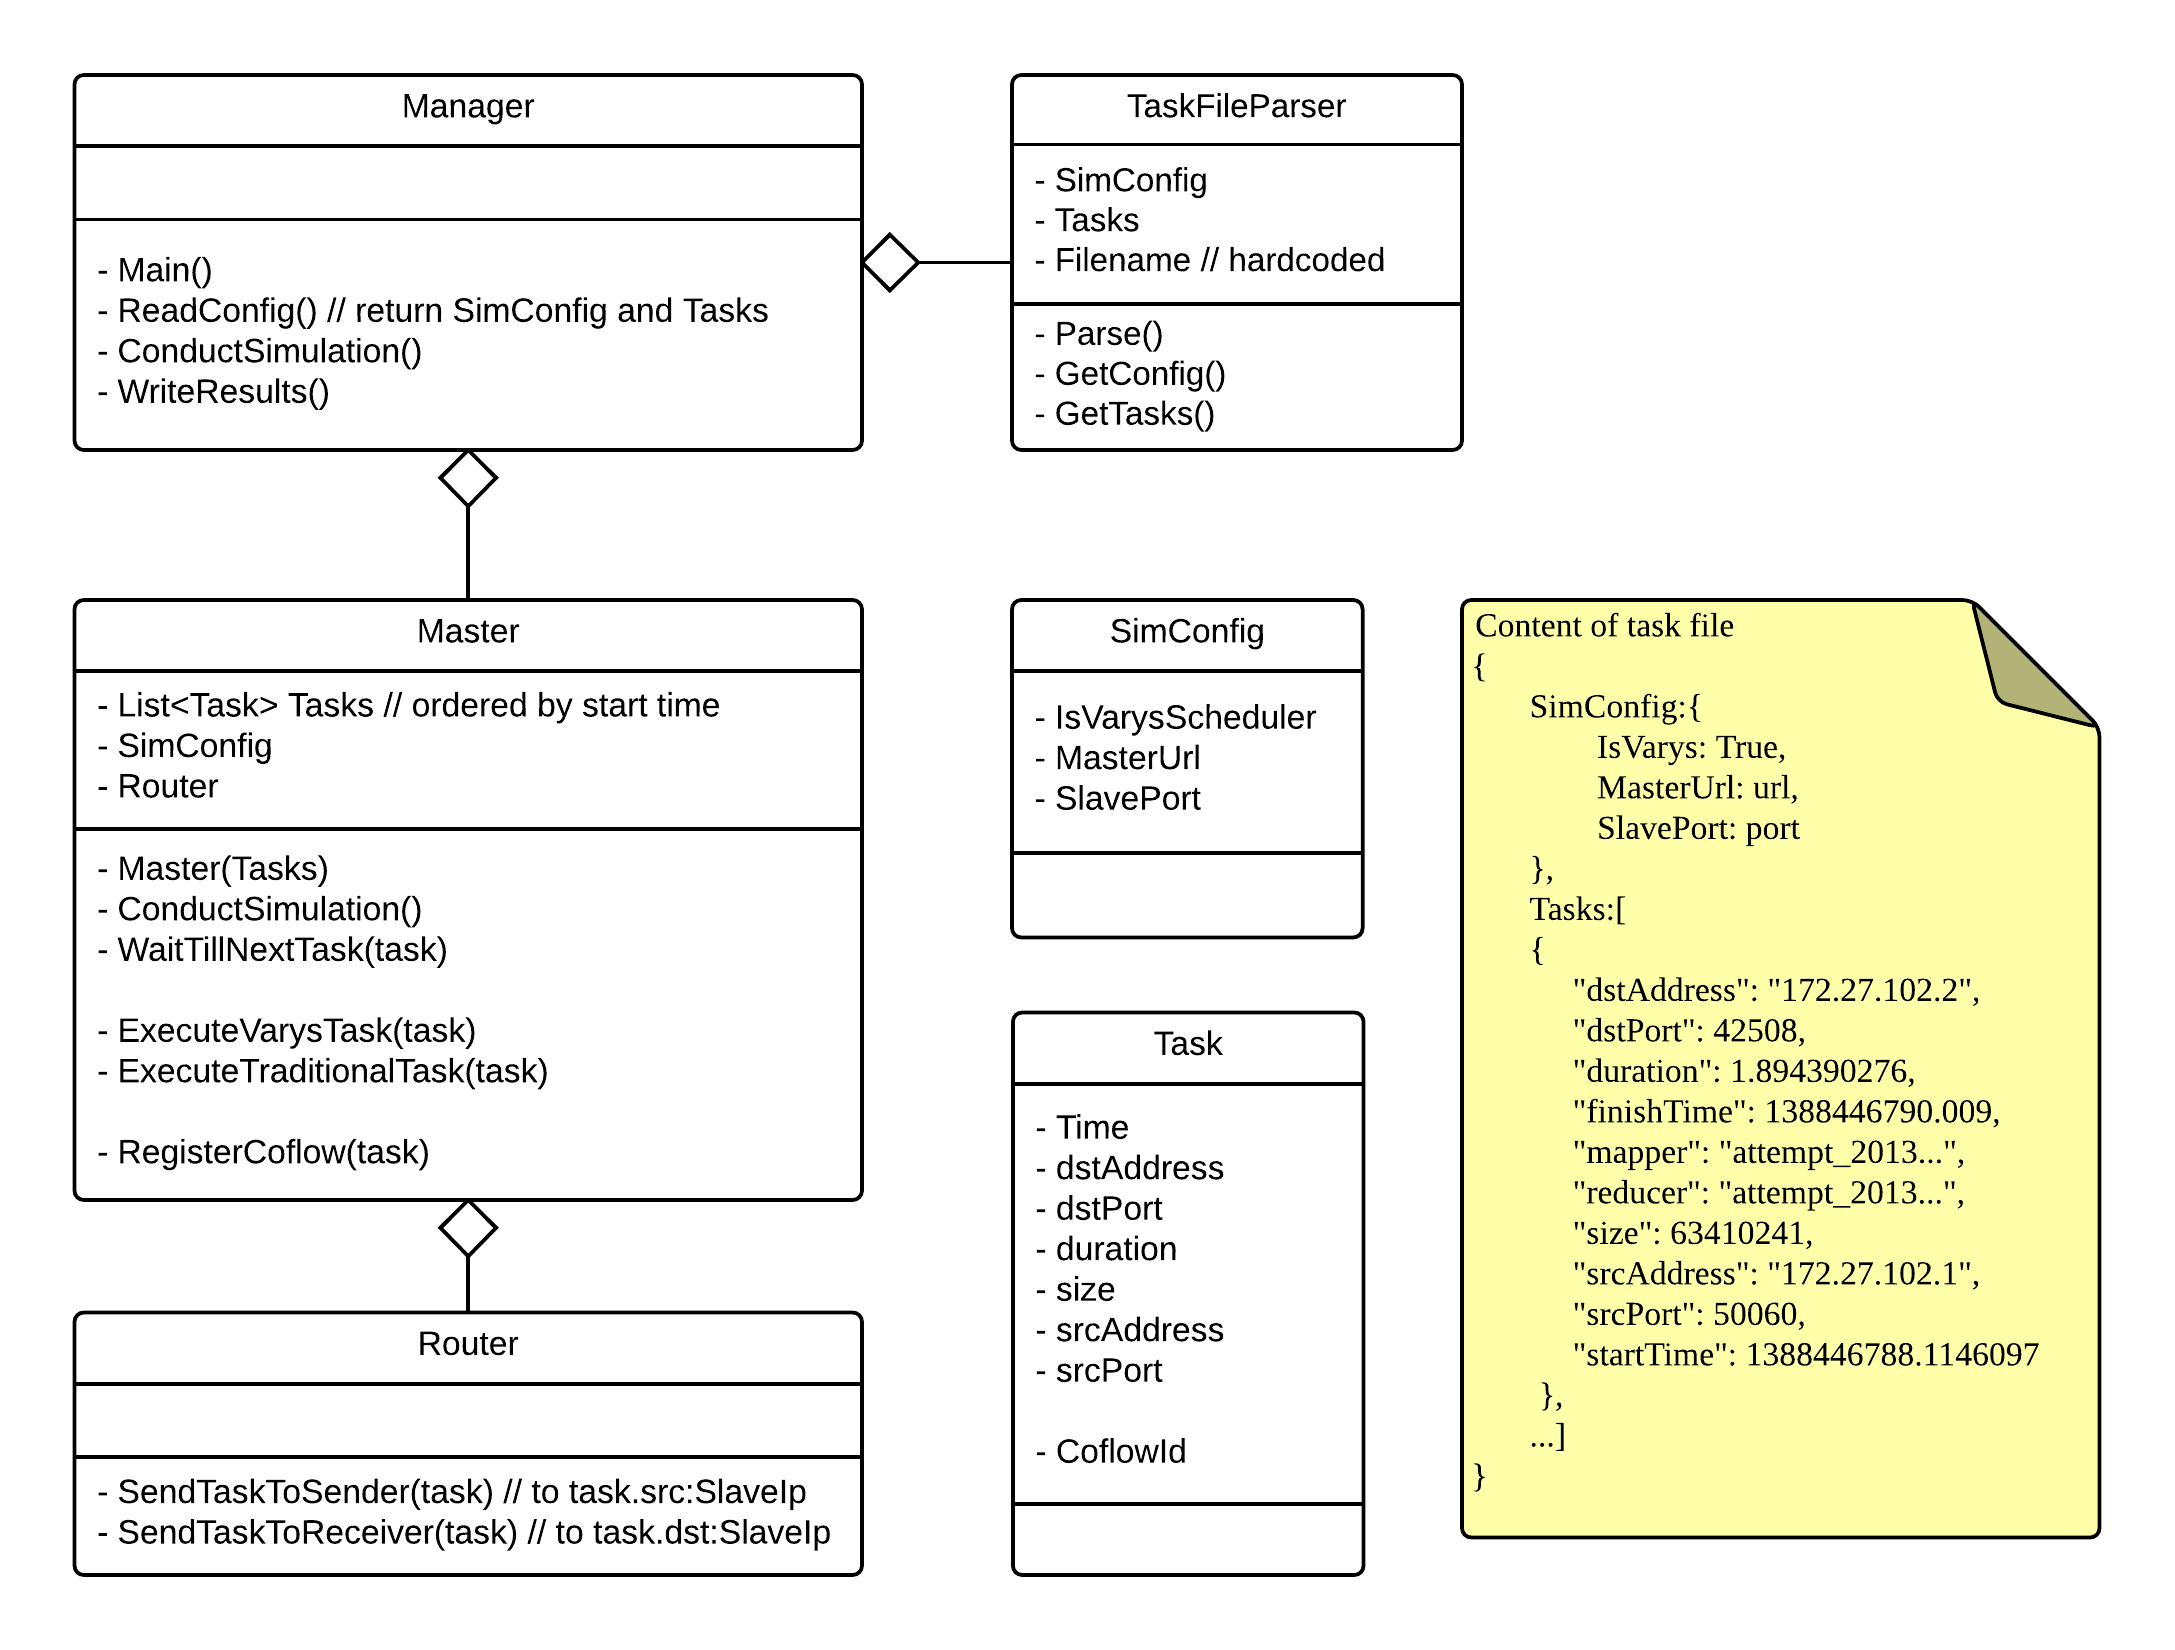
\includegraphics[scale = 0.75]{master.png}
\subsection{Slave}
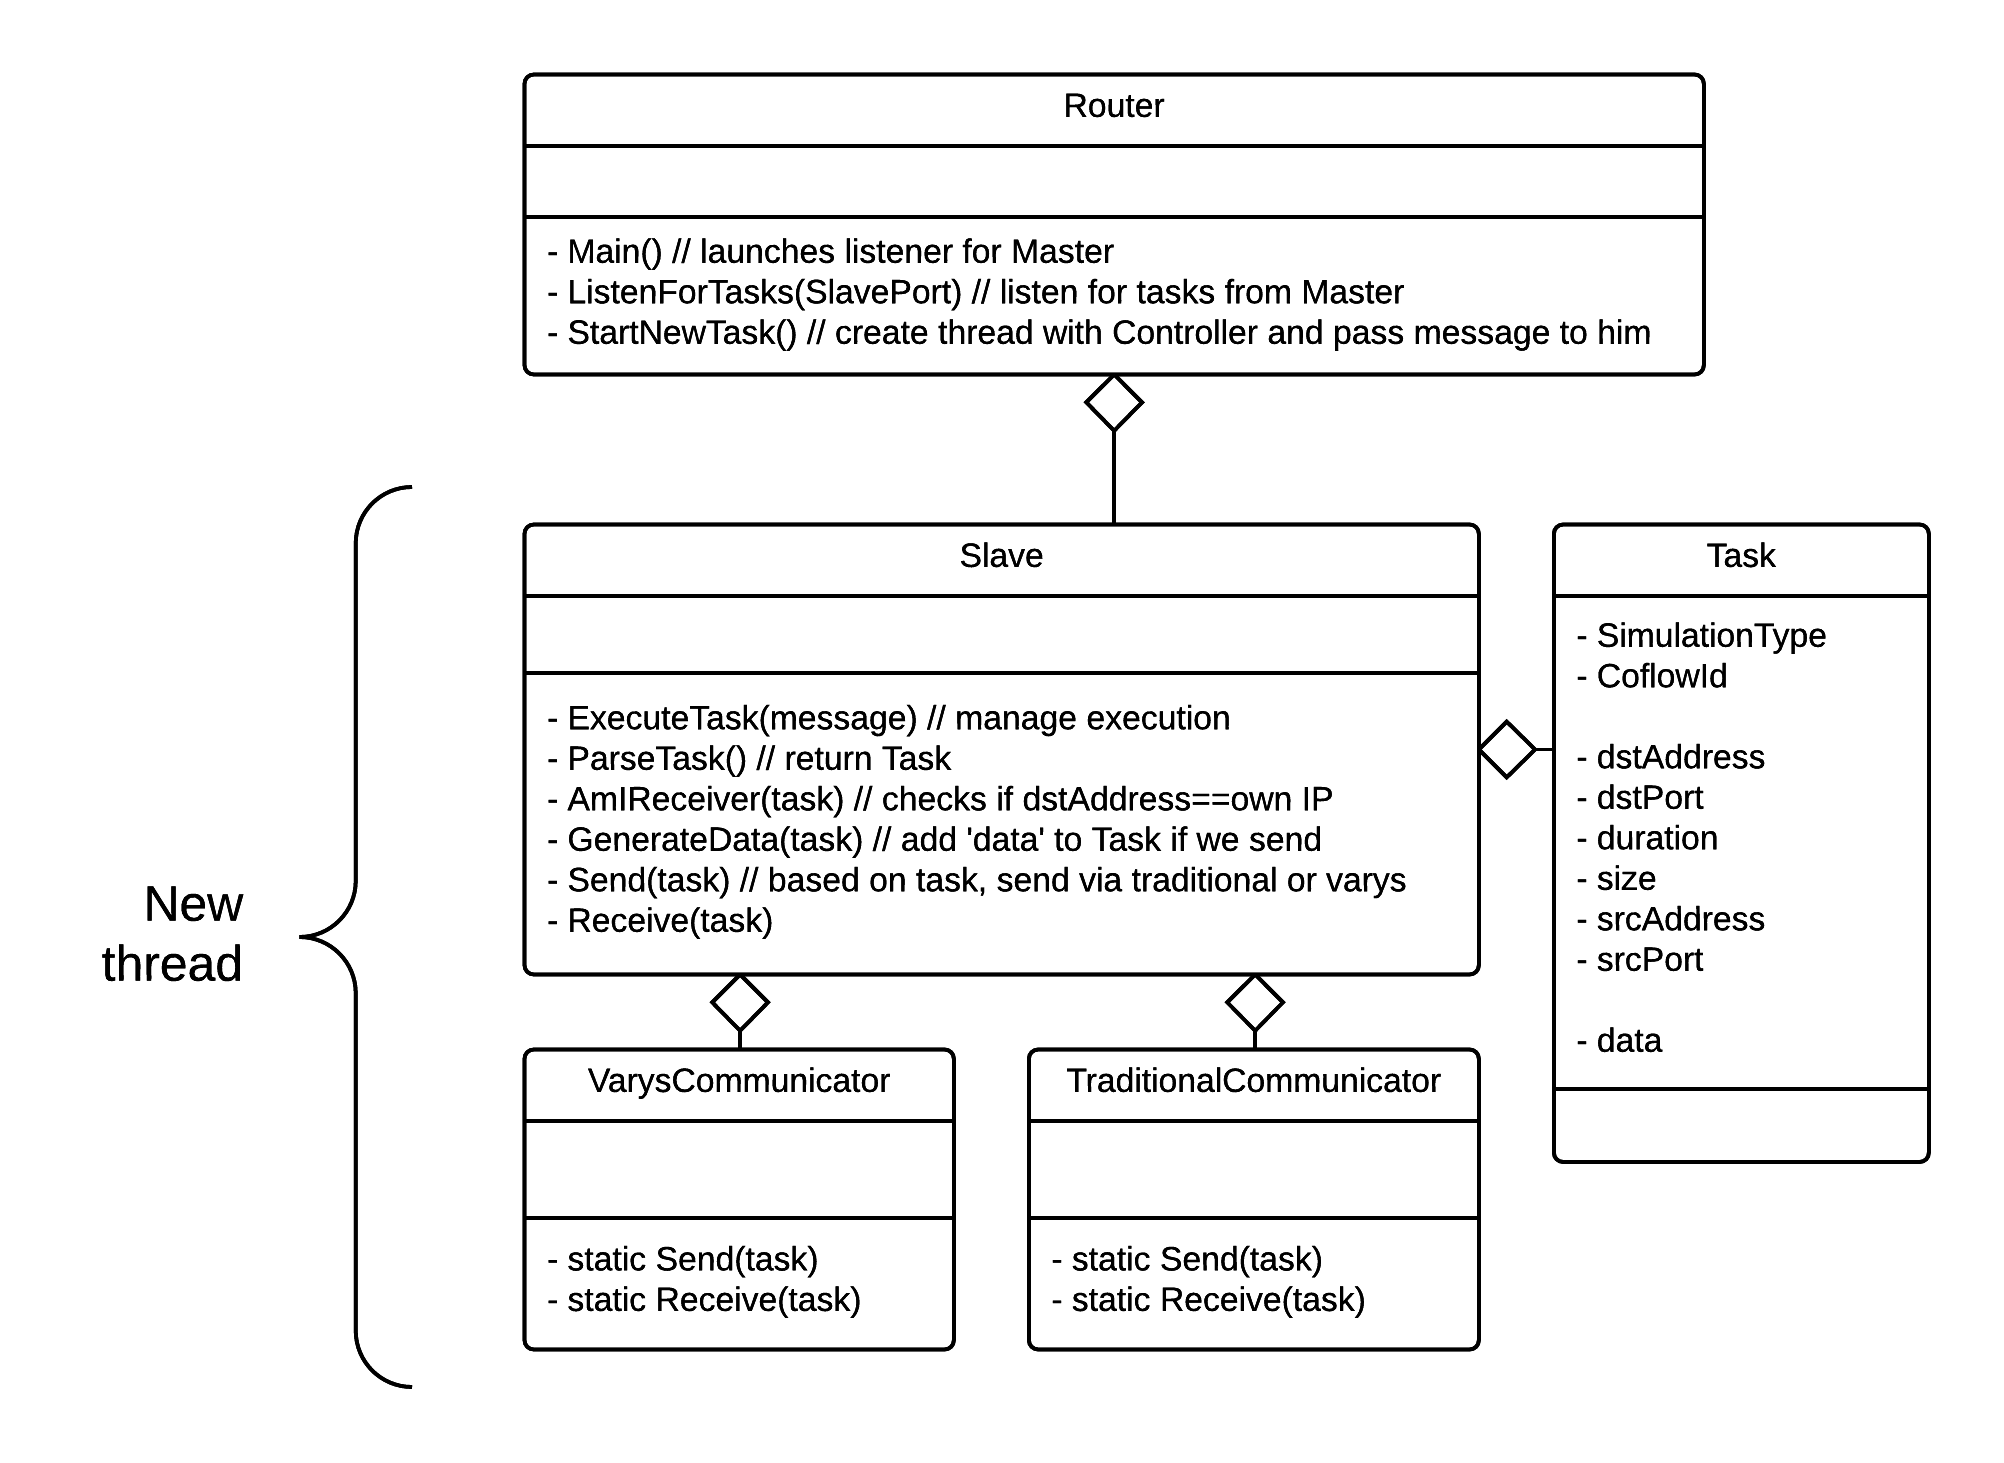
\includegraphics[scale = 0.75]{slave.png}

\section{Next Steps}
Below are the set of pending tasks for the project:
\begin{itemize}
	\item To get varys scheduling running on multiple mininet hosts, with the controller, mappers and reducers all running on different hosts.
	\item To run simulations using a realistic datacenter trace.
\end{itemize}

\bibliographystyle{plain}
\begin{thebibliography}{10}

\bibitem{mininet}
Mininet: An Instant Virtual Network \textit{mininet.org}

\bibitem{varys}
Efficient Coflow Scheduling with Varys, Mosharaf Chowdhury, Yuan Zhong, Ion Stoica, ACM SIGCOMM, 2014.

\bibitem{repo}
Team 06 Github Repo \textit{https://github.com/ucsdcse222a/group6}

\end{thebibliography}

\end{document}